\section{4 user study}
To demonstrate our proposed method, we investigated whether the level of experienced presence impacts the spatial exploration behavior of participants in a beyond room-scale VR. The \textit{invisible maze task} mimics a real-world exploration situation such as finding your way in complete darkness~\cite{Gehrke2018} (anonymized version attached). We conducted the following two-step analysis. First, we constructed parametric maps to assess where participants exploration behavior was impacted as a function of experienced presence. To this end, we investigated fine-grained behavior at each single point in space by conducting mass-univariate pixel-by-pixel modeling of experienced presence on duration spent at each location, i.e. pixel. We followed up on our findings with a classification scheme predicting experienced presence using participants characteristics such as video game experience and perspective taking ability, further details below. We considered a data-driven approach to finding a useful, i.e. scalable, classification model. Therefore, we initially included a variety of participant descriptors subsequently reducing them to a set with highest explanatory power. In this way, we hope to present a minimal model so other researchers may easily reproduce our findings. 

\subsection{Participants, Procedure, Task and Setup} Thirty-two healthy participants (aged 21--45 years, 14 men) took part in the experiment. All participants gave written informed consent to participation and the experimental protocol was approved by the local ethics committee (protocol: GR\_08\_20170428). Three participants were excluded from data analysis due to incomplete data or difficulties in complying with task requirements.

\begin{figure}[!t]
\centering
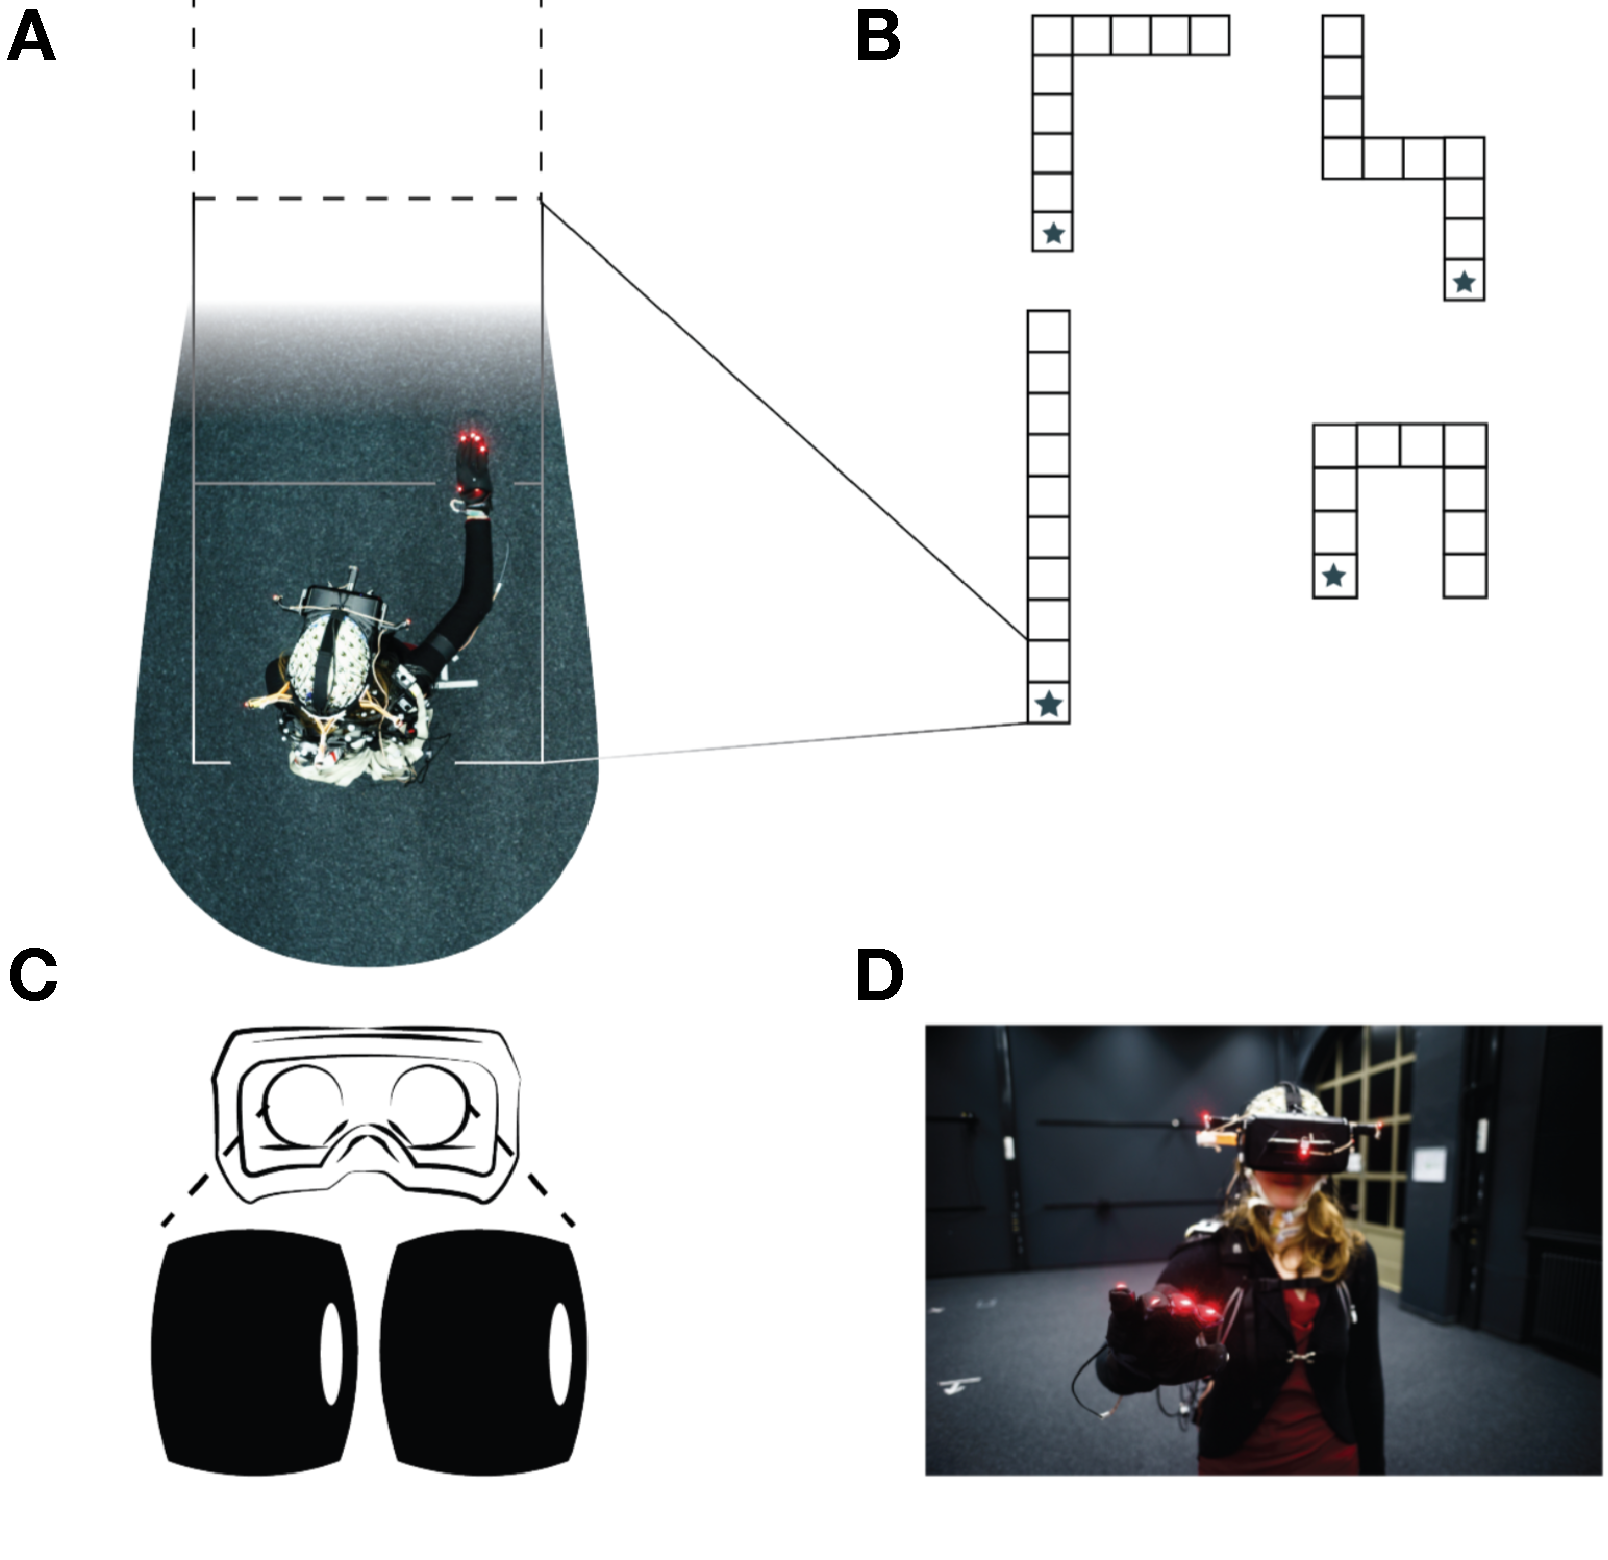
\includegraphics[width=\linewidth]{figures/IMT_Task.pdf}
\vspace{6pt}
\caption{Invisible Maze Task, \textbf{A,} Participant from a bird’s eye view. \textbf{B,} Participants are instructed to explore four different mazes and return to the start. \textbf{C,} First-person view in binocular `VR optics' of a wall touch. \textbf{D,} Participants were equipped with 160 channels wireless EEG, head-mounted virtual reality goggles and LEDs for motion capture. Find a detailed description in~\cite{Gehrke2018} (anonymized version attached).}
\label{imt_task}
\end{figure}

\subsubsection{The Invisible Maze Task} Participants freely explored a sparse invisible maze environment interactively by walking and probing for visual feedback when touching the virtual wall of a 1m wide path with their \textit{right} hand. All stimuli were presented using an Oculus Rift DK2 VR headset which was adaptable to be incorporated with the dedicated optical tracking system. Further the DK2 headset offered benefits regarding weight and modifiability. Upon collision of the \textit{right} hand with an invisible wall, a white disc was displayed 30 cm behind the collision point parallel to the invisible wall much like the beam form a torch in a cave, see figure \ref{imt_task} C (consult~\cite{Gehrke2018} (anonymized version attached) for extensive details on the task, instrumentation, and data collection). We did not track the left hand and instructed participants to keep the left arm close to their body. Performing the task, participants explored four different mazes in the order, `I', `L', `Z' and `U', see figure \ref{imt_task} B. The task was designed to emphasize participants internal build-up of a spatial representation of the maze layout. Doing the task, participants display a behavior that is comparable to explorative wall touches in the dark to find your way.

For each maze the procedure was as follows: participants were briefly disoriented and then positioned facing the open side of the path. Then, participants were directed to explore the invisible path until they reached a dead end, and subsequently find their way back to the starting position. At the end of each maze trial, participants received a gamified feedback and were then asked to draw a sketch map of the maze from a bird’s eye view as an index of spatial learning. The procedure was repeated three times in a row for each maze to foster spatial learning. For the present analysis, the three exploration phases were aggregated. The complete experiment, including preparation of physiological measures (Electroencephalogram, EEG) took approximately 4 hours. Preceding and following the task participants completed a set of questionnaires. We collected synchronized motion capture and behavioral events alongside high-density EEG.

\subsubsection{Assessing presence} To assess experienced presence, we administered the igroup presence questionnaire~\cite{Schubert2003}. For the reported analyses we considered only the first item of the questionnaire, the subjective presence measure (G1), which represents the sense of being in a place, i.e. `In the computer generated world I had a sense of "being there"' rated from `not at all' to `very much' on a 7-point Likert scale~\cite{Schubert2003, Slater1993}.